Thiết kế hướng miền cung cấp 2 loại mẫu:

\begin{itemize}

\item \textbf{Các mẫu chiến lược (Strategic Patterns):} Thiết kế phân chia một miền lớn và phức tạp thành các phần nhỏ hơn với ranh giới được xác định rõ ràng. Giúp phân chia một miền lớn hợp lý.

\item \textbf{Các mẫu kỹ thuật (Tactical Patterns):} Hiện thực hóa các mô hình khái niệm trong một thành phần nhỏ thành các thiết kế hệ thống phần mềm. Giúp hệ thống phù hợp với kinh doanh.

\end{itemize}


\begin{figure}[H]
    \centering
    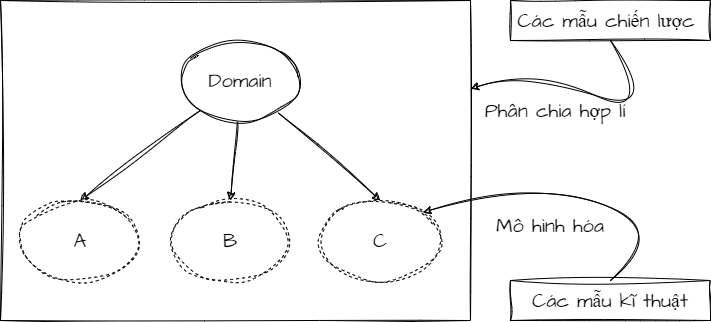
\includegraphics[width = 0.5\textwidth]{pictures/StrategicPatternsVATacticalPatterns/main.drawio.png}
    \caption{Khái quát tổng quan về Strategic Patterns và Tactical Patterns}
    \end{figure}

